% A literacy-free, report-free eye exam on a consumer EEG headband and a consumer
% VR headset, framed for mobile health. Two-page essentials version for IEEE ICCE.
\documentclass[conference]{IEEEtran}
\setlength{\textfloatsep}{0.6\baselineskip plus 0.2\baselineskip minus 0.2\baselineskip}
\setlength{\floatsep}{0.4\baselineskip plus 0.2\baselineskip minus 0.1\baselineskip}
\setlength{\abovecaptionskip}{2pt}
\IEEEoverridecommandlockouts
\usepackage{cite}
\usepackage{amsmath,amssymb}
\usepackage{graphicx}
\usepackage{url}
\usepackage[hidelinks]{hyperref}
\graphicspath{{figures/}}

\begin{document}

\title{A Literacy-Free, Report-Free Eye Exam on a Consumer EEG Headband and VR Headset:\\ Toward Objective Vision Screening by Community Health Workers}

\author{
\IEEEauthorblockN{Alexander Vicol and Steve Mann}
\IEEEauthorblockA{University of Toronto and MannLab Canada, Toronto, Canada}
% TODO: add co-authors and confirm affiliations before submission
}

\maketitle

\begin{abstract}
At least a billion people have a vision impairment that could be corrected, and the bottleneck is the screen: an eye test needs a literate, cooperating subject and a trained examiner. We describe an exam that asks nothing of the subject but to look at a dot with one eye covered, on a Muse headband with one electrode added over the visual cortex and a Meta Quest 3S running the stimulus in its browser, under 600 US dollars together. Acuity, vernier offset, contrast and its function over three bar widths, field, gaze, four meridians, red/green flicker photometry, colour and the apparent latency come from the steady-state visual evoked potential: an exact test per step, the sweep-VEP threshold rule, a fitted photometric null and the slope of the response phase over flicker rate. A hardware-free phantom with set cut-offs, a dead quadrant, an astigmatic axis and a red-weak eye passes all thirty-nine checks of a full-stack gate. Three sittings on a person were null, and the rig's own records found why: the headset's browser had kept a cached page from before the flash test, so the flicker was logged but never shown. With the page verified, a fourth sitting gave a flash response in both eyes on the occipital electrode, each eye's best flicker rate and one acuity limb; it also showed that a contact rule written for loose electrodes had discarded a responding one, and that the latency fit is ambiguous in its turn count. A fifth, with the ears in contact, took the right eye's acuity limb to 6~arcmin and found a response at every gaze position, and twice lost the phone's stream ten minutes in while the exam carried on blind; pausing on stream loss is now method. Nothing here is a diagnosis.
\end{abstract}

\begin{IEEEkeywords}
mobile health; visual screening; SSVEP; sweep VEP; wearable sensors; consumer electronics; community health workers.
\end{IEEEkeywords}

\section{The screen, not the lens, is the bottleneck}
The WHO counts at least 2.2 billion people with a vision impairment, at least a billion of them addressable, uncorrected refractive error first among the causes \cite{who2019vision}. A letter chart needs a subject who can read it in the examiner's language and an examiner to judge the answers. The pattern that has carried other screens to community health workers is a consumer device, a worker, and software that checks itself \cite{anand2018pulmonary,fletcher2010wearable}. The steady-state visual evoked potential (SSVEP) gives an objective acuity test with a clinical pedigree, the sweep VEP built for infants, who cannot report \cite{norcia1985sweep}, and a contrast threshold \cite{campbell1970contrast}; it removes literacy, language and examiner bias while bringing biases of its own in hair and headband fit \cite{fletcher2020fairness}.

\begin{figure}[t]
\centering
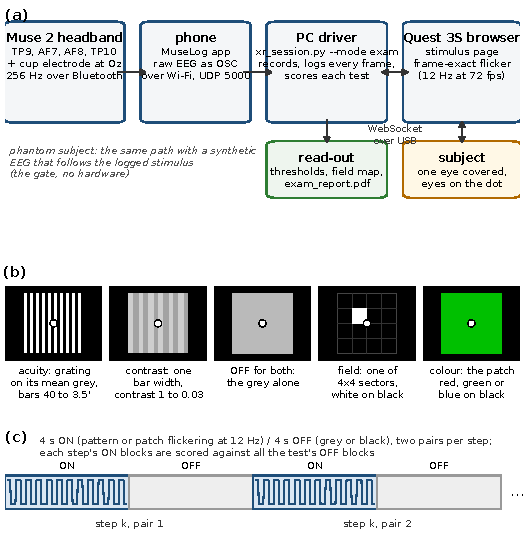
\includegraphics[width=0.9\columnwidth]{exam_diagram.pdf}
\caption{(a)~Scalp to read-out: the headband streams through the phone to the PC, which drives the page in the headset's browser, logs every frame and scores each test; the phantom replaces the first two boxes with a synthetic EEG that follows the logged stimulus. (b)~The four stimuli and the OFF screen of the grating tests. (c)~One step's blocks.}
\label{fig:diagram}
\end{figure}

\section{The rig and the exam}\label{sec:rig}
Mann et~al.\ turned the eye into a camera with the SSVEP \cite{mann2019eye}; we rebuilt that rig on a Muse headband with a cup electrode at Oz, the phone streaming raw EEG as the hub in the wireless-sensing architecture iCalm set out \cite{fletcher2010icalm}, and a Quest 3S whose browser renders the stimulus (Figs.~\ref{fig:diagram}, \ref{fig:photos}). Every stimulus fills the window: the camera runs had shown the response grows with the flickering area and a small square gives nothing. Each eye opens with the window flickering white/black, the camera's calibration stimulus (five ON/OFF pairs of 4~s at 12~Hz on the 72~Hz display), which must respond and whose channel and amplitude are the reference for the eye's tests. The flash then runs at six rates, 6 to 36~Hz: amplitude against rate is the eye's temporal tuning, the slope of phase against rate its apparent latency \cite{regan1966}, whose difference between the eyes is the clinical pattern VEP's measure. Then, two pairs per step: a grating whose bars swap places at the flicker rate, each resolved bar swinging like the flash at a constant mean luminance (pattern reversal \cite{norcia1985sweep}), 40 to 3.5~arcmin (acuity) or contrast 1 to 0.03 (contrast); one quadrant at a time (field); the whole window again while the dot sits at the centre and then 84\% of the way to each edge, so the flicker falls to one side of the fovea (gaze); the window red, green or blue (colour). Four tests were added after the fourth sitting. Coarse bars cut into strips three bars high, every other strip jumping sideways by an offset and back at the flicker rate against the aligned bars as OFF, the offset shrinking from 8 to 0.5~arcmin and delivered to a quarter of a device pixel by the canvas's own anti-aliasing: the vernier VEP, a hyperacuity that amblyopia degrades more than acuity \cite{norcia1999vernier}. The contrast sweep again at 60 and 10~arcmin, which with its 20-arcmin point gives three points of the contrast sensitivity function. The grating at 14~arcmin turned to 0, 45, 90 and 135 degrees, where a weak meridian beside a strong one at right angles is the signature of astigmatism. And heterochromatic flicker photometry \cite{wagner1972photometry}: a red field and a green field exchanged at the flicker rate, the pair's luminance held while red's share runs from 0.2 to 0.8, with the steady mixture of the two as OFF so neither the mean luminance nor the chromaticity changes; the luminance response has its null where the two fields are equally bright to this eye, so the red share at the null is the eye's isoluminant point, 0.5 for the display's standard observer and higher for a red-weak eye, and the response left there is the chromatic pathway's. The null is fitted as $a\,M(s;p_0)+b$ over $p_0$, $M$ the exchange's luminance modulation for an eye whose fields match at share $p_0$, rather than read off the dimmest step. Each step's ON blocks are scored against all the test's OFF blocks by the line power at the flicker frequency and its double, with an exact permutation test over the channels in contact. Contact has two tiers: a channel above 300~$\mu$V rms through a test is open or railing and is set aside; between 60 and 300~$\mu$V it is noisy and kept only if its own ON/OFF test is significant. Thresholds follow the sweep-VEP rule: a line through the limb from the step below the finest responding one up the rise, extrapolated to zero; two asked widths the panel delivers as one are one step. The delivered stimulus is verified, not assumed: the page is served uncacheable at a fresh URL each sitting, its code is fingerprinted through the browser's debug port before the trigger, and the headset's own frame buffer is captured during a block. About fifteen minutes per eye with the eleven tests; the seven of the fourth sitting take nine, and the driver takes any subset.

\begin{figure}[t]
\centering
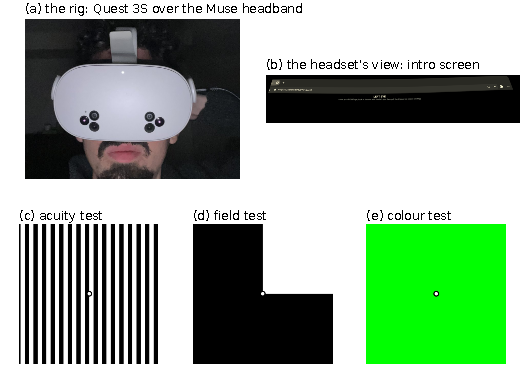
\includegraphics[width=0.66\columnwidth]{exam_photos.pdf}
\caption{(a)~The Quest 3S over the Muse headband. (b)~The headset's own view of one eye's intro screen. (c)--(e)~The page during an ON frame of the acuity, field and colour tests.}
\label{fig:photos}
\end{figure}

\section{Validation without a patient}
A device for a worker with no eye clinic behind them must be testable with no patient in front of it. A phantom subject reads the stimulus log as it is written and streams synthetic EEG whose SSVEP follows what is on screen, through a logistic visibility in bar width and contrast with a cut-off per eye, dead quadrants, colour gains, and a latency and a flicker cut per eye. The gate dials in a right eye at 8~arcmin and contrast 0.08 with one dead quadrant, 120~ms late and holding to 40~Hz, a left eye twice as coarse and whole, 150~ms late and half gone by 24~Hz, gains 0.7/1/0.4 for red/green/blue, and asks twenty-five things: every stage delivered, the flash responding in both eyes on Oz and every test read on it, each threshold inside the band where the phantom's visibility runs from 0.02 to 0.6, the left eye at least $1.3\times$ coarser, exactly the dead quadrant named, every gaze position responding, green~$\geq$~red~$>$~blue, every rate responding, the half rate and the latencies within 15\% and 6~ms of the dialled. All twenty-five pass (Fig.~\ref{fig:gate}): right eye 3.8~arcmin, contrast 0.029, quadrant 3 silent, 108~ms, still over half at 30~Hz; left eye 7.8~arcmin and 0.082, half rate 22.5~Hz, 30~ms later than the right; every gaze position 0.90 to 0.98 of the centre in both eyes. The gate earns its keep on every change: the first run with the gaze test failed exactly its two checks, because the phantom follows a fixed list of stimulus logs and the new one was not on it. The four later tests brought dials of their own, a vernier cut-off per eye (1 and 2~arcmin), an astigmatic axis and gain for the right eye (0.4 of full along the horizontal bars, rising as $\cos^2$ to full for vertical) and a red-weak left eye whose fields match at a red share of 0.65 against the right's 0.5, with a tenth of the response left at the null, and fourteen more checks, thirty-nine in all (Fig.~\ref{fig:gatenew}): both vernier thresholds in their bands (0.37 and 0.88~arcmin) and the left at least $1.3\times$ the right; every contrast threshold of the csf test inside the contrast band at both of its bar widths; the right eye's weakest meridian at 90 degrees, at 0.47 of the best, and the left's four within 0.90 of each other; the nulls at 0.49 and 0.65, their difference $+0.16$. The vernier sweep is also the proof that the page delivers sub-pixel offsets: the right eye's response fell from full at 2~arcmin through half at 1 to nothing at 0.5, the dialled logistic.

\begin{figure}[t]
\centering
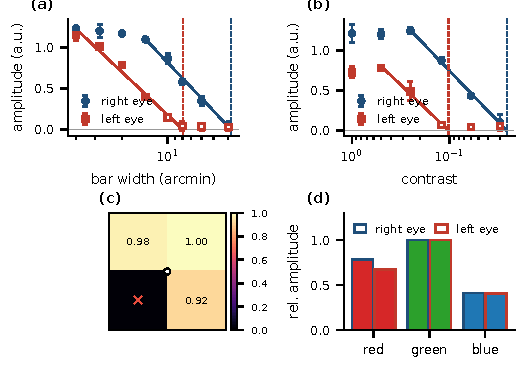
\includegraphics[width=0.6\columnwidth]{exam_gate.pdf}
\caption{The gate's read-out. (a)~Acuity and (b)~contrast per phantom eye (right circles, left squares; open: $p \geq 0.05$), fitted limbs and their zero crossings. (c)~The right eye's field, the cross its dead quadrant. (d)~Colour planes.}
\label{fig:gate}
\end{figure}

\begin{figure}[t]
\centering
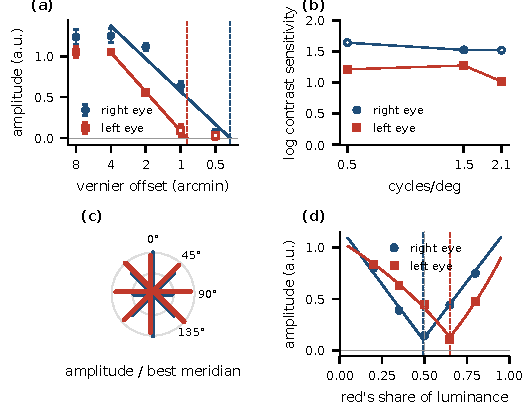
\includegraphics[width=0.98\columnwidth]{exam_gate_new.pdf}
\caption{The gate's read-out of the four tests added after the fourth sitting (right circles, left squares; open: $p \geq 0.05$). (a)~Vernier: amplitude against the strips' offset, the fitted limbs and their zero crossings. (b)~The contrast sensitivity function from the three bar widths. (c)~Meridians: each orientation's amplitude over the best (right eye blue, left red); the right eye's dialled weak axis is the horizontal one. (d)~Flicker photometry: amplitude against red's share of the luminance, the fitted null model and the nulls, the display's match dotted.}
\label{fig:gatenew}
\end{figure}

\section{Five sittings on a person}
One of the authors ran the exam four times on one day, right eye then left, at 12~Hz, and a fifth time the day after. The first three fitted nothing. The first taught the contact check: both ear electrodes had sat at 100 to 280~$\mu$V rms, loose under the headset strap, and the signal check, written for electrodes at the amplifier rails, had passed them, the quiet failure a consumer wearable brings to the field \cite{fletcher2010wearable}; the exam now measures every channel before each eye and tells the subject which pad to press. The cause of all three surfaced in the fourth, in the headset's own frame buffer: during an ON block the view was black but for the dot, and the page's code, read through the browser's debug port, lacked the flash test. The browser had kept a cached copy of the page from a build before it, while the driver logged 72 frames per second of flicker from the page it thought it had. A logged stimulus is not a shown one; hence the delivery checks of Section~\ref{sec:rig}.

\begin{figure}[t]
\centering
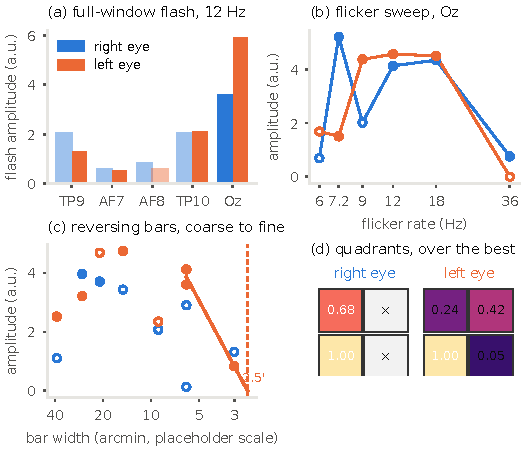
\includegraphics[width=0.98\columnwidth]{exam_human.pdf}
\caption{The fourth sitting, both eyes on the occipital cup. (a)~The flash per channel: right eye $p = 0.024$, left $p = 0.008$; hatched bars not significant. (b)~The sweep: the right eye peaks at 7.2~Hz and is half gone by 8, the left peaks at 12 and holds to 25. (c)~Reversing bars: the left eye responds to 6~arcmin and not to 3, the limb crossing at 2.5 on the headset's placeholder pixel scale; the right eye only to 21 and coarser. (d)~Quadrants: the same pattern in both eyes, which points at the electrode, not the retinas.}
\label{fig:human}
\end{figure}

With the current page the fourth sitting measured (Fig.~\ref{fig:human}): a flash response on the occipital electrode in both eyes, right $p = 0.024$ at line SNR 9.6, left $p = 0.008$ at 18; a best rate of 7.2~Hz in the right eye and 12~Hz in the left, so the session rate suited one eye and not the other; bars resolved to 6~arcmin by the left eye, a limb extrapolating to 2.5~arcmin at the placeholder scale, against 21~arcmin by the right; no contrast limb in either; the same quadrant pattern in both eyes, bottom-left strongest and bottom-right weakest or silent, the signature of one electrode sitting off the midline between the two calcarine banks rather than of two retinas; and colour ratios that agree between the eyes (R:G:B 0.69:1:0.18 and 0.72:1:0.26), mostly the display's primaries, since a colour test proper exchanges two colours at equal luminance. Two methods changed on this data. The left eye had first been read on a forehead channel: its occipital electrode sat at 105~$\mu$V rms and the 60~$\mu$V rule set it aside, yet block by block it carried the sitting's strongest line, SNR 6 to 18 in every ON block against under 1.5 in every OFF block; hence the two tiers of Section~\ref{sec:rig}. And the apparent latencies, 77~ms right and 258~ms left, differ by a turn of phase, not by physiology: the phase step from 12 to 18~Hz is 209$^\circ$ in one eye and 197$^\circ$ in the other, and the fit took different turn counts because the eyes responded at different rate sets. The latency is reported as undetermined until the fit shares its turn count across the eyes, and the between-eye difference, the number the test exists for, needs both eyes responding at the same rates.

The fifth sitting ran the eleven tests on the right eye. Its flash was the strongest yet (3.0, $p = 0.004$); the sweep peaked at 18~Hz and held to 27, where the day before the same eye had peaked at 7.2 and been half gone by 8, so the tuning is not yet a stable measure of the eye; the bars responded down to 6~arcmin with the limb crossing at 2.7 on the placeholder scale, against 21 the day before, the gain of an electrode that held; and the whole window responded at every gaze position, 0.3 to 0.9 of the centre. The vernier offsets, the contrast steps and the csf gave no limb: the occipital cup sat in the noisy tier through those minutes and the vernier fell back to a forehead channel. Twice, about ten minutes after the phone began to stream, its stream stopped, and the driver carried on through five tests with no EEG before the operator noticed; the lost tests were run again in a second session with its own flash, and the read-out joins the two. Two more lessons for the method: the exam must pause when its stream goes and resume when it returns, and a test read on an electrode that has fallen into the noisy tier must be repeated, not carried.

\section{What the same recording carries}
A headband records more than the visual response \cite{picard1997affective}. In companion sittings on the same rig the forehead electrodes gave the blink rate, which stops while a patch flickers, bursts when it goes dark, and doubled between two sittings of one evening, an old marker of fatigue \cite{stern1994blink}: the hook for a just-in-time adaptive intervention \cite{nahum2018jitai}, an eye-strain estimate against the subject's own earlier minutes, not detection and not emotion.

\section{Toward the field}
Established: the apparatus, an exact test per step, the sweep-VEP threshold rule, the latency from the phase slope, the photometric null, a phantom gate of thirty-nine checks that catches failures without a volunteer, and on one person a flash response in both eyes, each eye's best rate, an acuity limb to 6~arcmin and a response at every gaze position. Not established: a threshold in physical units, since the headset's pixels per degree is unmeasured; a latency free of its turn-count ambiguity; a vernier, contrast or photometric reading on a person, which the sittings so far have not held the occipital electrode steady enough to give, and whose absolute photometric null carries the display's unmeasured primaries; a stream that survives a sitting, or an exam that pauses when it does not; and any reading of the quadrants until the electrode sits on the midline. Open after those: a blur study with trial lenses against a letter chart, a normative cohort, and a worker-facing flow with the report as one picture.

\bibliographystyle{IEEEtran}
\bibliography{refs}

\end{document}
